\section{Theorie}

In diesem Versuch soll Röntgenemission und -absorption analysiert werden.

Um Röntgenstrahlen zu erzeugen wird eine evakuierte Röhre benötigt, in welcher
Elektronen, die aus einer Glühkathode emittiert werden, durch ein Elektrisches
Feld beschleunigt werden. Die kinetische Energie der Elektronen ist dabei
$E_\text{kin} = e \cdot U$, wobei $e$ die Elementarladung ist.

Daraufhin treffen die Elektronen auf eine Anode, wobei die Röntgenstrahlung
entsteht. Die Strahlung setzt sich aus dem kontinuierlichen Bremsspektrum und
der charakteristischen Röntgenstrahlung zusammen.

Das kontinuierliche Bremsspektrum entsteht, wenn die Elektronen durch das Coulombfeld
der Atome des Anodenmaterials abgebremst werden. Die Photonen haben dabei die Energie,
die das Elektron verliert. Das Bremsspektrum ist kontinuierlich, da das Elektron
beliebig viel Energie durch die Abbremsung verlieren kann. Es gibt allerdings
eine minimale Wellenlänge die das Photon bei dem Bremsspektrum haben kann.

\begin{equation}
  \lambda_\text{min} = \frac{hc}{eU}
  \label{eq:1}
\end{equation}

Das charakteristische Spektrum wird erzeugt, wenn ein Atom aus dem Anodenmaterial
so ionisiert wird, dass ein Elektron aus einer inneren Schale herausgelößt wird.
Dann kann ein Elektron aus einer äußeren Schale den leeren Platz einnehmen. Bei
diesem Vorgang wird ein Photon ausgesendet. Die Energie dieses Photons ist gerade
die Energiedifferenz der beiden Energieniveaus $E_m - E_n$. Aus diesem Grund ist das
charakteristische Spektrum ein Linienspektrum.

Bei Mehrelektronenatomen muss bei der Bestimmung der Energieniveaus noch eine
korrektur vorgenommen werden, da die Elektronenhüllen die Kernladung abschirmen.
Damit ergibt sich für die Bindungsenergie eines Elektrons aus der n-ten Schale:

\begin{equation}
  E_n = - R_\infty z_\text{eff}^2 \frac{1}{n^2}.
  \label{eq:2}
\end{equation}

Dabei ist $z_\text{eff} = z - \sigma$ die effektive Kernladung, wobei $\sigma$
die Abschirmkonstante ist und $R_\infty = \SI{13.6}{\eV}$ ist die
Rydbergenergie. \\\\

Wenn die erzeugten Röntgenstrahlen von einem anderen Material absorbiert werden,
treten verschiedene Effekte auf.

\begin{figure}
  \centering
  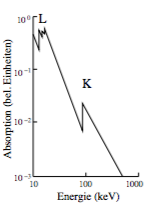
\includegraphics[width=0.38\textwidth]{content/Absorption.png}
  \caption[width=\linewidth]{Beispielgraphik zur Absorption von Röntgenstrahlung \cite{1}.}
  \label{abb:1}
\end{figure}

Wie in der Abbildung \ref{abb:1} gezeigt wird, nimmt der Absorptionskoeffizient
mit zunehmender Energie ab. Aber er steigt sprunghaft an, wenn die Energie des Photons
und die Bindungsenergie des Elektrons aus einer Schale ungefähr gleich sind.
In der Abbildung \ref{abb:1} wird auch deutlich, dass es drei L-Absorptionskanten
gibt, das liegt an der Feinstruktur. Aus diesem Grund muss für die Bestimmung der
Bindungsenergien die \enquote{Sommerfeldsche Feinstrukturformel} verwendet werden.

\begin{equation}
  E_{n,j} = - R_\infty \left( z_\text{eff,1}^2 \frac{1}{n^2} + \alpha^2
  z_\text{eff,2}^4 \frac{1}{n^3} \left( \frac{1}{j+\frac{1}{2}} - \frac{3}{4n}
  \right)\right)
  \label{eq:3}
\end{equation}

Dabei ist $\alpha$ die Sommerfeldsche Feinstrukturkonstante, n die Hauptquantenzahl
und j der Gesamtdrehimpuls.

Nun lässt sich auch die Abschirmkonstante $\sigma_L$ aus den L-Absorptionskanten
bestimmen indem die Energiedifferenz zweier L-Kanten bestimmt wird.

\begin{equation}
  \sigma_L = Z - \left( \frac{4}{\alpha} \sqrt{\frac{\Delta E_L}{R_\infty}}
  - \frac{5 \Delta E_L}{R_\infty} \right)^{\frac{1}{2}} \left(
  1 + \frac{19}{32} \alpha^2 \frac{\Delta E_L}{R_\infty} \right)^{\frac{1}{2}}
  \label{eq:4}
\end{equation}

Bei diesem Versuch wird die Energiedifferenz aus $\Delta E_L = E_{L_2} - E_{L_3}$
bestimmt.

Um die Wellenlänge der Röntgenstrahlung bestimmen zu können wird die Bragg´sche
Reflexion verwendet. Dabei werden die Photonen auf ein Atomgitter, zum Beispiel
ein Kristall, geleuchtet und dabei werden sie an jedem Atom gebeugt. Unter einem
bestimmten Winkel, den Glanzwinkel $\theta$, ergibt sich konstruktive Interferenz.
Nun kann mit der Bragg´schen Bedingung durch diesen Winkel die Wellenlänge bestimmt werden.

\begin{equation}
  \lambda = \frac{2d \sin(\theta)}{n}
  \label{eq:5}
\end{equation}

Dabei ist d die Gitterkonstante und n die Beugungsordnung.
